\chapter{构建端盖三维模型}\label{chap:duangai}

{\bfseries 学习目标}
\begin{itemize}
\item 学习利用fillet命令绘制连接圆弧
\item 学习利用filletedge命令构建三维圆弧
\end{itemize}

{\bfseries 任务要求}
\begin{itemize}
\item 根据图\ref{fig:tiaoyafaduangai}所示的杯零件图,用旋转法建立调压阀杯零件的三维模型
\item 根据图\ref{fig:tiaoyafaduangai}所示的杯零件图,用实体建模法建立调压阀杯零件的三维模型
\end{itemize}

\noindent
\begin{figure}[htbp]
\centering
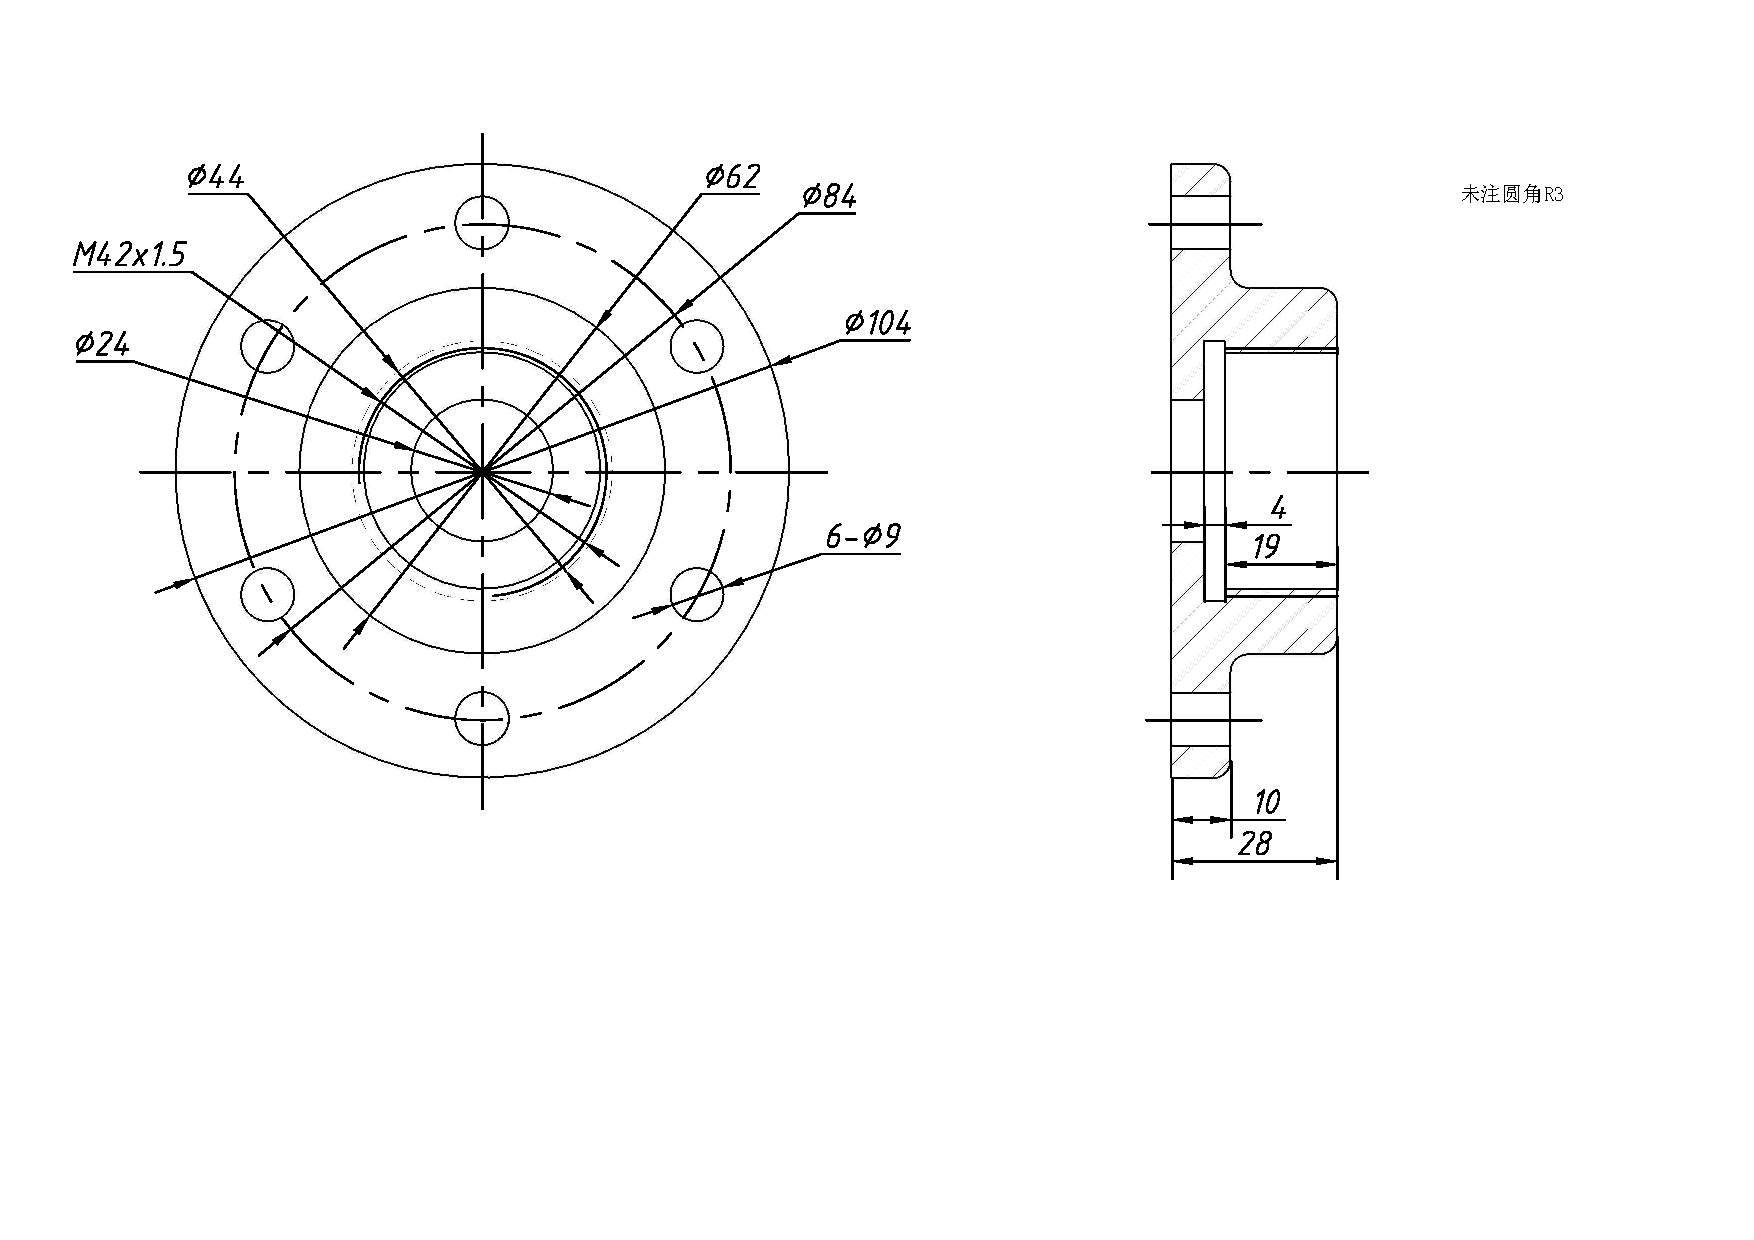
\includegraphics[scale=0.5]{tiaoyafaduangai.pdf}
\caption{端盖零件图}\label{fig:tiaoyafaduangai}
\end{figure}
\clearpage
\section{截交体与相贯体的三视图}
\subsection{截交体}
 机器零件通常需要加工一些斜切口或开槽,这些结构可以看作是一个或多个平面切割立体而成。通常将这类立体称之为截交体。
 \subsubsection{棱柱截交体}
 图\ref{fig:jiejiao1}为正六边形棱柱截交体。该截交体的截交平面与$V$面垂直,其截交平面在俯视图和左视图中为类似形的五边形,其三视图投影如图\ref{fig:jiejiao2}所示。
 \begin{figure}[htbp]
 \centering
\subfloat[]{\label{fig:jiejiao1}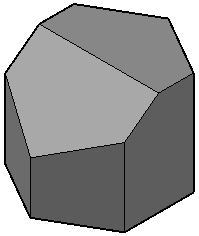
\includegraphics[scale=0.8]{jiejiao1.png}}\hspace{30pt}
\subfloat[]{\label{fig:jiejiao2}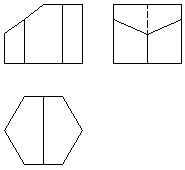
\includegraphics[scale=1]{jiejiao2.png}}
\caption{正六棱柱截交体}
\end{figure}
\subsubsection{棱锥截交体}
 图\ref{fig:jiejiao3}为正三边形棱柱截交体。该截交体的截交平面由平行于$H$面和垂直于$V$面的截交面构成,其三视图投影如图\ref{fig:jiejiao4}所示。
 \begin{figure}[htbp]
 \centering
\subfloat[]{\label{fig:jiejiao3}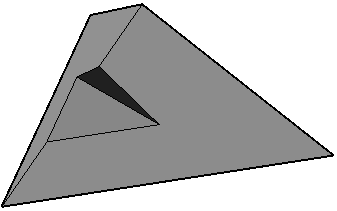
\includegraphics[scale=0.6]{jiejiao3.png}}\hspace{30pt}
\subfloat[]{\label{fig:jiejiao4}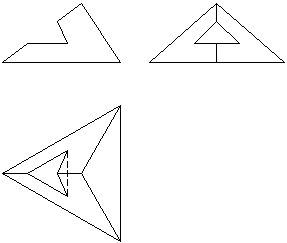
\includegraphics[scale=0.65]{jiejiao4.png}}
\caption{正六棱柱截交体}
\end{figure}
\subsubsection{圆柱截交体}
 \begin{figure}[htbp]
 \centering
\subfloat[]{\label{fig:jiejiao5}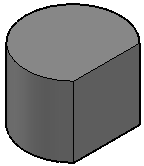
\includegraphics[scale=0.8]{jiejiao5.png}}\hspace{60pt}
\subfloat[]{\label{fig:jiejiao6}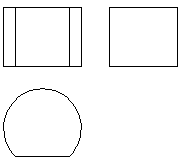
\includegraphics[scale=0.8]{jiejiao6.png}}\\
\subfloat[]{\label{fig:jiejiao7}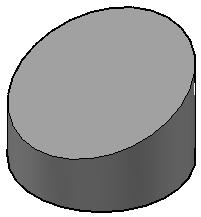
\includegraphics[scale=0.6]{jiejiao7.png}}\hspace{60pt}
\subfloat[]{\label{fig:jiejiao8}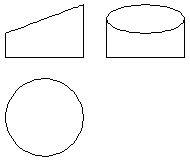
\includegraphics[scale=0.8]{jiejiao8.png}}\\
\subfloat[]{\label{fig:jiejiao9}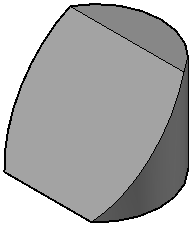
\includegraphics[scale=0.6]{jiejiao9.png}}\hspace{60pt}
\subfloat[]{\label{fig:jiejiao10}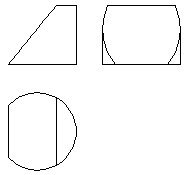
\includegraphics[scale=0.9]{jiejiao10.png}}
\caption{圆柱截交体}
\end{figure}
图\ref{fig:jiejiao5}为截交平面与轴线平,其截交线为一矩形,图\ref{fig:jiejiao6}是其三视图;图\ref{fig:jiejiao7}为截交面倾斜于轴线且不与上下表面相交,其截交线为一椭圆,图\ref{fig:jiejiao8}是其三视图;图\ref{fig:jiejiao9}为截交平面倾斜于轴线且与上下表面相交,其截交线为为复合图形,图\ref{fig:jiejiao10}是其三视图。
\clearpage
\subsubsection{圆锥截交体}
 \begin{figure}[htbp]
 \centering
\subfloat[]{\label{fig:jiejiao11}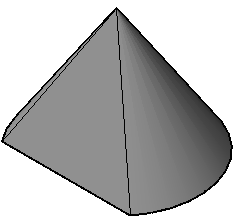
\includegraphics[scale=0.45]{jiejiao11.png}}\hspace{60pt}
\subfloat[]{\label{fig:jiejiao12}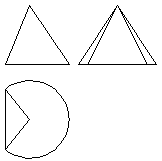
\includegraphics[scale=0.65]{jiejiao12.png}}\\
\subfloat[]{\label{fig:jiejiao13}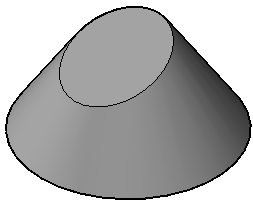
\includegraphics[scale=0.45]{jiejiao13.png}}\hspace{60pt}
\subfloat[]{\label{fig:jiejiao14}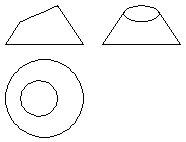
\includegraphics[scale=0.65]{jiejiao14.png}}\\
\subfloat[]{\label{fig:jiejiao15}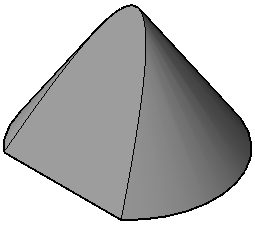
\includegraphics[scale=0.45]{jiejiao15.png}}\hspace{60pt}
\subfloat[]{\label{fig:jiejiao16}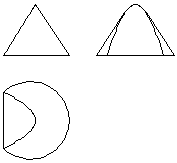
\includegraphics[scale=0.65]{jiejiao16.png}}\\
\subfloat[]{\label{fig:jiejiao17}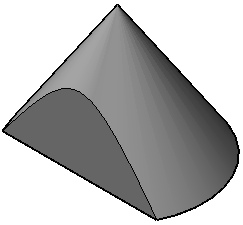
\includegraphics[scale=0.45]{jiejiao17.png}}\hspace{60pt}
\subfloat[]{\label{fig:jiejiao18}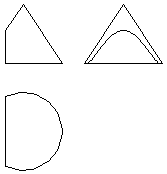
\includegraphics[scale=0.65]{jiejiao18.png}}
\caption{圆锥截交体}
\end{figure}
图\ref{fig:jiejiao11}为截交面通圆锥体锥顶,其截交线为三角形,图\ref{fig:jiejiao12}为其三视图;图\ref{fig:jiejiao13}为截面倾斜于轴线且倾斜角度大于锥角,其截交线为椭圆,图\ref{fig:jiejiao14}为其三视图;图\ref{fig:jiejiao15}为截面倾斜于轴线且倾斜角度等于锥角,其截交线为抛物线,图\ref{fig:jiejiao16}为其三视图;图\ref{fig:jiejiao17}为截面与轴线平行,其截交线为双曲线,图\ref{fig:jiejiao18}为其三视图。
\endinput
 
\section{旋转建模法}
\subsection{绘制左视图特征图}
\begin{procedure}
\item 设置图层。

建立“中心线”和“实线”两个图层,分别用于管理中心线和实线两类图形,并将图层设置为“中心线”层。
\item 切换视图为左视图。

\item 绘制左视图中心线。

绘制两条相互垂直的构造线型中心作为绘图参考线
\begin{lstlisting}
|命令: XLINE|
|指定点或 [水平(H)/垂直(V)/角度(A)/二等分(B)/偏移(O)]: 0,52|
|指定通过点:$ @1<0$|
|指定通过点:$ @1<90$|
|指定通过点:|
\end{lstlisting}
偏移产生$\phi 9$圆的中心线
\begin{lstlisting}
|命令: OFFSET|
|当前设置: 删除源=否  图层=源  OFFSETGAPTYPE=0|
|指定偏移距离或 [通过(T)/删除(E)/图层(L)] $<$通过$>$:42|
|选择要偏移的对象,或 [退出(E)/放弃(U)] $<$退出$>$:|
|指定要偏移的那一侧上的点,或 [退出(E)/多个(M)/放弃(U)] $<$退出$>$:|
|选择要偏移的对象,或 [退出(E)/放弃(U)] $<$退出$>$:|
\end{lstlisting}
\item 将图层切换为实线图层,绘制忽略连接圆弧的特征图,其结果如图\ref{fig:duanguaitezhengtu}所示。
\begin{figure}[htbp]
\centering
\subfloat[]{\label{fig:duanguaitezhengtu}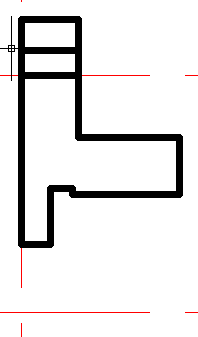
\includegraphics[scale=0.62]{duanguaitezhengtu.png}}\hspace{30pt}
\subfloat[]{\label{fig:duanguaitezhengtu1}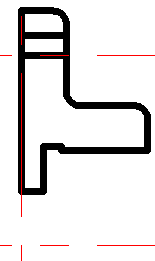
\includegraphics[scale=0.75]{duanguaitezhengtu1.png}}
\caption{端盖左视特征图绘制过程}
\end{figure}
绘主特征图。
\begin{lstlisting}
|命令: line|
|指定第一个点: 0,64|
|指定下一点或 [放弃(U)]: @0,40|
|指定下一点或 [放弃(U)]: @10,0|
|指定下一点或 [闭合(C)/放弃(U)]: @0,-21|
|指定下一点或 [闭合(C)/放弃(U)]: @18,0|
|指定下一点或 [闭合(C)/放弃(U)]: @0,-10|
|指定下一点或 [闭合(C)/放弃(U)]: @-19,0|
|指定下一点或 [闭合(C)/放弃(U)]: @0,1|
|指定下一点或 [闭合(C)/放弃(U)]: @-4,0|
|指定下一点或 [闭合(C)/放弃(U)]: @0,-10|
|指定下一点或 [闭合(C)/放弃(U)]: c|
\end{lstlisting}
绘制$\phi 9$孔特征图。
\begin{lstlisting}
|命令: rectang|
|指定第一个角点或 [倒角(C)/标高(E)/圆角(F)/厚度(T)/宽度(W)]:|
|指定另一个角点或 [面积(A)/尺寸(D)/旋转(R)]: @10,4.5|
\end{lstlisting}
\item 绘制圆弧连接,其结果如\ref{fig:duanguaitezhengtu1}所示。

绘制圆弧外连接的通常使用圆角命令。启动圆角命令的方法有:
\begin{itemize}
\item 键盘输入FILLET\index{fillet}或F。
\item 【修改】$\rightarrow$【圆角】。
\item 【修改】$\triangleright$【圆角】图标
\includegraphics[scale=0.6]{fillet.png}。
\end{itemize}
启动圆角命令后,要求选择对象。通常情况下,第一次启动圆角命令,其半径值为零。因此需要使用【半径(R)】选项先设置半径。
\begin{lstlisting}
|命令: fillet|
|当前设置: 模式 = 修剪,半径 = 0.0000|
|选择第一个对象或 [放弃(U)/多段线(P)/半径(R)/修剪(T)/多个(M)]: r| 
\end{lstlisting}
输入半圆角半径值。
\begin{lstlisting}
|指定圆角半径 $<$0.0000$>$: 3|
\end{lstlisting}
选择用于生成圆角的两边。
\begin{lstlisting}
|选择第一个对象或 [放弃(U)/多段线(P)/半径(R)/修剪(T)/多个(M)]:|
|选择第二个对象,或按住 Shift 键选择对象以应用角点或 [半径(R)]:|
\end{lstlisting}
用相同的方法生成其余两个圆角。由于圆角半径是一致的,因此不需要重复设置圆角半径,只需要直接选择用于圆角的边即可。
\begin{lstlisting}
|命令: FILLET|
|当前设置: 模式 = 修剪,半径 = 3.0000|
|选择第一个对象或 [放弃(U)/多段线(P)/半径(R)/修剪(T)/多个(M)]:|
|选择第二个对象,或按住 Shift 键选择对象以应用角点或 [半径(R)]:|
|命令: FILLET|
|当前设置: 模式 = 修剪,半径 = 3.0000|
|选择第一个对象或 [放弃(U)/多段线(P)/半径(R)/修剪(T)/多个(M)]:|
|选择第二个对象,或按住 Shift 键选择对象以应用角点或 [半径(R)]:
\end{lstlisting}
\item 面域特征图。
\begin{lstlisting}
|命令: region|
|选择对象: 指定对角点: 找到 12 个|
|选择对象:|
\end{lstlisting}
\end{procedure}
圆角命令的注意事项和技巧:
\begin{tips}
\item 如果圆角半径值为零,则不会生成圆角。
\item 圆角命令用于绘制三段圆弧内连接不是很方便,建立用使用圆或者圆弧命令,通过捕捉切点来完成。
\end{tips}

\endinput
\subsection{旋转法构建端盖三维模型}
\begin{procedure}
\item 切换西南等轴测图

\item 旋转构建端盖三维模型
旋转产生$\phi 9$圆柱体。
\begin{lstlisting}
|命令: revolve|
|当前线框密度:  ISOLINES=4,闭合轮廓创建模式 = 实体|
|选择要旋转的对象或 [模式(MO)]: MO 闭合轮廓创建模式 [实|
|体(SO)/曲面(SU)] $<$实体$>$: SO|
|选择要旋转的对象或 [模式(MO)]: 找到 1 个|
|选择要旋转的对象或 [模式(MO)]:|
|指定轴起点或根据以下选项之一定义轴 [对象(O)/X/Y/Z] $<$对象$>$:|
|指定轴端点:|
|指定旋转角度或 [起点角度(ST)/反转(R)/表达式(EX)] $<$360$>$:|
\end{lstlisting}
旋转产生端盖主特征三维模型,其结果如图\ref{fig:duangai1}所示。

\begin{lstlisting}
|命令: revolve|
|当前线框密度:  ISOLINES=4,闭合轮廓创建模式 = 实体|
|选择要旋转的对象或 [模式(MO)]: MO 闭合轮廓创建模式 [实|
|体(SO)/曲面(SU)] $<$实体$>$: SO|
|选择要旋转的对象或 [模式(MO)]: 找到 1 个|
|选择要旋转的对象或 [模式(MO)]:|
|指定轴起点或根据以下选项之一定义轴 [对象(O)/X/Y/Z] $<$对象$>$:|
|指定轴端点:near 到|
|指定旋转角度或 [起点角度(ST)/反转(R)/表达式(EX)] $<$360$>$:|
\end{lstlisting}
\item 三维阵列$\phi 9$圆柱体,其结果如图\ref{fig:duangai2}所示。
\begin{lstlisting}
|命令: 3darray|
|选择对象: 找到 1 个|
|选择对象:|
|输入阵列类型 [矩形(R)/环形(P)]$<$矩形$>$:p|
|输入阵列中的项目数目: 6|
|指定要填充的角度 (+=逆时针, -=顺时针)$ <360>$:|
|旋转阵列对象? [是(Y)/否(N)] $<Y>$:|
|指定阵列的中心点:|
|指定旋转轴上的第二点:|
\end{lstlisting}
\begin{figure}[htbp]
\centering
\subfloat[]{\label{fig:duangai1}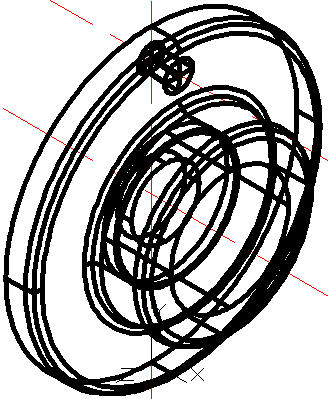
\includegraphics[scale=0.45]{duangai1.png}}\hspace{30pt}
\subfloat[]{\label{fig:duangai2}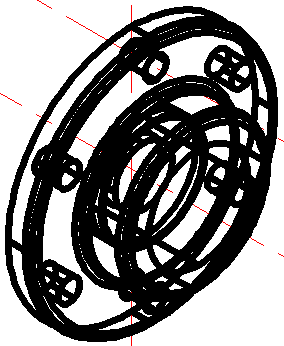
\includegraphics[scale=0.5]{duangai2.png}}\hspace{30pt}
\subfloat[]{\label{fig:duangailititu}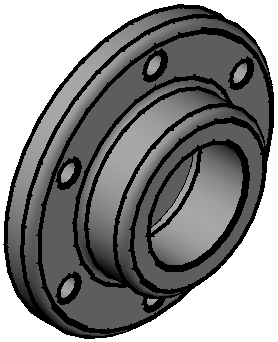
\includegraphics[scale=0.5]{duangailititu.png}}
\caption{端盖三维模型构建过程}
\end{figure}
\item 用差集操作完成三维建模操作。
\begin{lstlisting}
|命令: subtract |
|选择要从中减去的实体、曲面和面域...|
|选择对象: 找到 1 个|
|选择对象:  选择要减去的实体、曲面和面域...|
|选择对象: 找到 1 个|
|选择对象: 找到 1 个,总计 2 个|
|选择对象: 找到 1 个,总计 3 个|
|选择对象: 找到 1 个,总计 4 个|
|选择对象: 找到 1 个,总计 5 个|
|选择对象: 找到 1 个,总计 6 个|
|选择对象:|
\end{lstlisting}
\item 设置视觉样式为真实,其结果如图\ref{fig:duangailititu}所示。
\item 将端盖模型保存为“调压阀端盖立体图.dwg”。
\end{procedure}
\section{轴承支座立体图}

\endinput
\endinput